\documentclass{article}[a4paper,12pt]
\usepackage[utf8]{inputenc}
\usepackage{amsmath,amssymb,amsthm,amsfonts,mathtools}
\usepackage[inline]{enumitem}
\usepackage{soul}
\usepackage{cancel}
\usepackage{hyperref}
\usepackage{centernot}
\usepackage{pifont}
\usepackage{changepage}
\usepackage{subcaption}
\usepackage[section]{placeins}
\usepackage{lipsum, graphicx, caption}
\usepackage{float}
\usepackage{commath}
\usepackage{wrapfig}
\usepackage{amsmath}
\usepackage{amsfonts}
\usepackage{amssymb}
\theoremstyle{definition}
\newtheorem{innercustomgeneric}{\customgenericname}
\providecommand{\customgenericname}{}
\newcommand{\newcustomtheorem}[2]{%
  \newenvironment{#1}[1]
  {%
   \renewcommand\customgenericname{#2}%
   \renewcommand\theinnercustomgeneric{##1}%
   \innercustomgeneric
  }
  {\endinnercustomgeneric}
}
\newcustomtheorem{customthm}{Theorem}
\newcustomtheorem{customlem}{Lemma}
\newcustomtheorem{customdefn}{Definition}
\newcustomtheorem{customprop}{Proposition}
\newcustomtheorem{customexer}{Exercise}
\renewcommand{\qedsymbol}{$\blacksquare$}

\setlength\parindent{0pt}
\let\emptyset\varnothing
\usepackage{geometry}
\geometry{
	a4paper, portrait,
	total = {170mm,257mm},
	left = 20mm,
	top = 20mm,
}

\usepackage{xcolor}
\usepackage{pagecolor}
\pagecolor{white}
\color{black}

\title{\textbf{Introduction to Game Developement}}
\author{
	\textbf{Om Prabhu}\\
	19D170018\\
	Undergraduate, Department of Energy Science and Engineering\\
	Indian Institute of Technology Bombay\\}
\date{Last updated \today}

\begin{document}
\maketitle
\vspace{-12pt}
\hrulefill
\vspace{6pt}

\textbf{NOTE:} This document is a brief compilation of my notes taken during a course in game design and development. You are free to use it and my project files for your own personal use \& modification. You may check out the course here: \texttt{\href{https://www.coursera.org/learn/game-development?specialization=game-development}{https://www.coursera.org/learn/game-development?specialization=game-development}}.

\hrulefill
\tableofcontents
\pagebreak

\section{Introduction}
\subsection{About myself}
Hello. I am Om Prabhu, currently an undergrad at the Department of Energy Science and Engineering, IIT Bombay. If you have gone through my website (\texttt{\href{https://omprabhu31.github.io}{https://omprabhu31.github.io}}) earlier, which is probably where you found this document too, you will know that I love playing video games, story-rich titles in particular. I also listen to a lot of music and engage in a little bit of creative writing as and when I get time. With this brief self-introduction, let's get into what actually motivated me to pursue game development.

\subsection{Motivation}
Most of my motivation for pursuing game development came from playing games itself. I am talking less of titles like \textit{Grand Theft Auto}, generic FPS/RPGs, etc meant purely for self-entertainment and more about games like \textit{Life is Strange}, \textit{When the Darkness Comes}, etc that actually give you some amazing stories and/or simple, powerful messages to be remembered for life. When one has experiences like this, the question naturally hangs at the back of their minds - why not create enriching experiences like this?
\vspace{6pt}

Now while playing games (of all genres) is vital to understanding what essentially makes a good game, they are two very different things - it's like comparing movie binging to actually making movies. Making games involves a lot of hardwork at different stages of the development process and there is a reason why good game developers take their time (often more than 10 years) before putting out a game on the market.
\vspace{12pt}

Nevertheless, I decided to give it a shot - the worst that could happen is I could end up hating it, but I hate it during quarantine anyway.

\hrulefill
\vspace{6pt}

\textbf{NOTE:} 
\begin{enumerate}
	\item This entire course works with Unity3D as the game engine, however the exact same concepts apply to other engines like Unreal, Godot, etc as well.
	\item Even if you are using a newer or older version of Unity, the concepts apply just as well. In fact, there is almost negligible difference in functionality between releases.
	\item The source files for course projects are available on my website for free use and modification. I will mainly be working with the 2019.4.2f1 and 2017.4.40f1 LTS releases of Unity, so you might need to install these versions of the engine before you try them out.
	\item Most of the project builds will be for the WebGL platform. Many browsers do not support running local WebGL content out of the box. You might find this guide handy: \texttt{\href{techwiser.com/enable-webgl}{techwiser.com/enable-webgl}}
	\item If you want to install Standard Assets through Unity Hub, then you might want to install a 2017 LTS release (Unity no longer releases Standard Assets from 2018). Otherwise there is always the option of importing and using 2017 Standard Assets in a 2018 or 2019 release.
\end{enumerate}
\hrulefill
\pagebreak

\section{Overview of Game Development}
\subsection{Factors to consider before starting out}
\begin{center}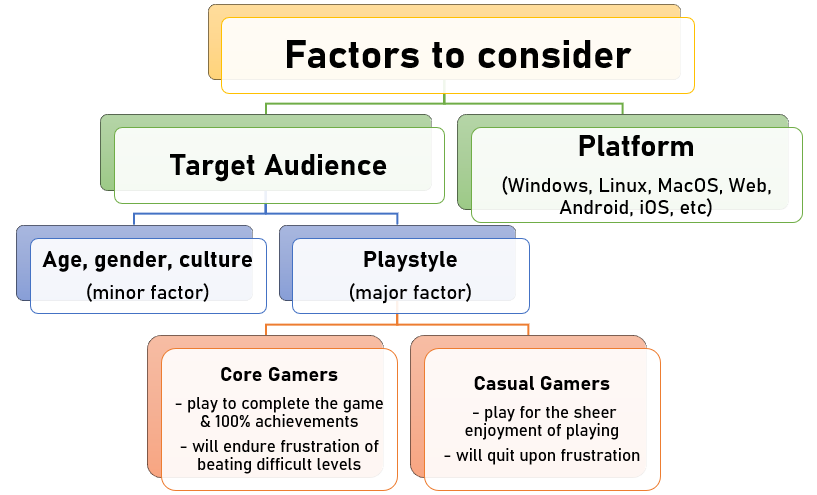
\includegraphics[scale=0.8]{gamedev_basic_factors_to_consider.png}\end{center}

\subsection{Hierarchy of game structure}
Keeping in mind the above factors, we proceed to conceptualize the game structure.
\begin{center}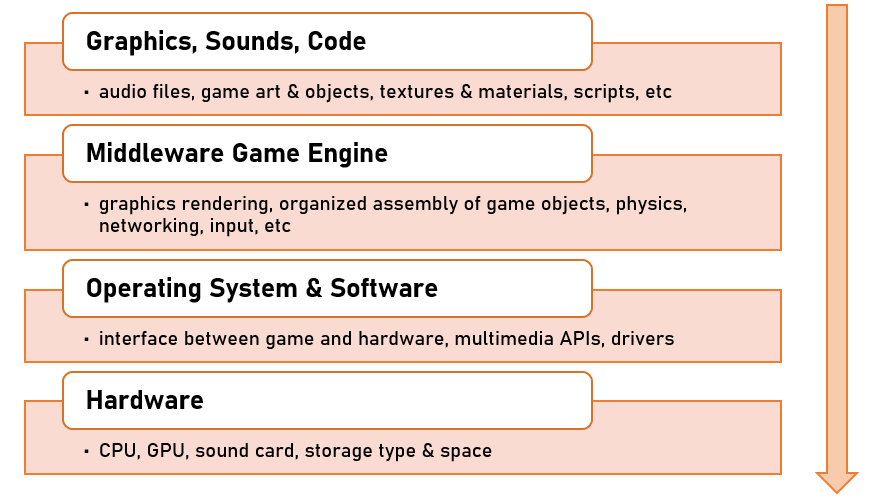
\includegraphics[scale=0.8]{game_design_hierarchy.png}\end{center}

While normally we would construct anything from the ground up, from a game design perspective things work better when conceptualized from the top down. 
\begin{itemize}
	\item We first create everything essential, i.e. `game assets' - that would mean any art, textures \& materials, game object models, audio/music and scripts (basically code that defines interaction between objects)
	\item Then, we actually construct the levels in the game using the above created assets in an engine like Unity, Unreal, Godot, etc
	\item We then build the game for the intended platforms
	\item Finally the game is tested for bugs and to determine the requirements for a system that could hope to run our game
\end{itemize}

\subsection{Team structure and roles}
Considering all the stuff from the previous subsection, it would be near impossible for a single person to carry out all the work required and make an end product that ticks all the boxes (individual developers do exist still). This is why there are often teams, ranging in size from as small as 2-3 people to well over 1000 employees, with each member having one or more roles to perform.
\begin{itemize}
	\item Game Designer: execution of the idea behind the story, designing levels, gameplay mechanics, organizing assets and documents
	\item Story Designer: character design, story arcs, writing dialogues, etc
	\item Game Producer: monitoring project budgets, keeping track of deadlines, keeping the team together
 	\item Programmer: writing actual code to determine how game objects interact
	\item Game Artist: create concept art, textures for game objects to give them unique looks 
	\item Sound Designer: create and edit music to match the mood of various in-game scenes
	\item Game Tester: not the same as a player; requires sitting on a single game level for hours to identify bugs/inconsistencies
\end{itemize}
Depending on the size of the team, each person may assume one or more of the above roles based on what they can best do:
\begin{itemize}
	\item a small team (1-5 people) may be able to make do with just general purpose designers, artists and programmers, and each person will be more or less actively involved in production work
	\item a medium sized team (6-25 people) may additionally require a manager/producer and specialized designers \& artists
	\item a large team (25+ people) will have supplementary roles like scripters (people who have knowledge of programming as well as design), technical artists (programmers who can also work as artists) and level designers (who make the artwork and game design for separate levels)
\end{itemize}
\hrulefill
\pagebreak

\section{The Unity3D Engine}
All games need a few basic features - loading and displaying game assets, playing sound FX. receive player input and react to it, some code to define game rules and mechanics. One way to incorporate all of this is to build everything from scratch i.e. the core game software, renderers, etc. While this can certainly be done, it is much easier to use a game engine to do most of the work for us.
\vspace{6pt}

A game engine is a platform that provides basic game functionality, support for integration of game objects of multiple different formats. This allows us to focus on the actual unique gameplay elements.
\vspace{6pt}

Some advantages of using the Unity3D game engine are:
\begin{itemize}
 	\item great documentation (by which I mean insanely great) and a very large dev community
	\item very fast build times and support for many platforms
	\item great asset pipeline (mechanism to import and use game assets)
	\item not as processor intensive as other engines like Unreal
	\item can actively switch between different editor versions using Unity Hub without needing to rebuild the entire project
\end{itemize}
\textbf{NOTE:} If you take up this course, the instructor will mention that Unity3D offers flexibility in programming languages between C\# and JavaScript. This is no longer valid after the 2019 LTS releases. However, many .NET compatible languages like C++ can be used if they are first compiled into a DLL (for which you can refer this - \texttt{\href{https://docs.unity3d.com/Manual/UsingDLL.html}{https://docs.unity3d.com/Manual/UsingDLL.html}}).
\subsection{Unity3D interface and configuration}
The process of downloading and installing Unity is very intuitive and I won't go over it. However, note that Unity has stopped distributing the Standard Assets Example Project from 2018 onwards, so you might need to use the 2017 releases if you want to try stuff out with the example project. On launching Unity, the editor window might look something similar to this:
\vspace{6pt}

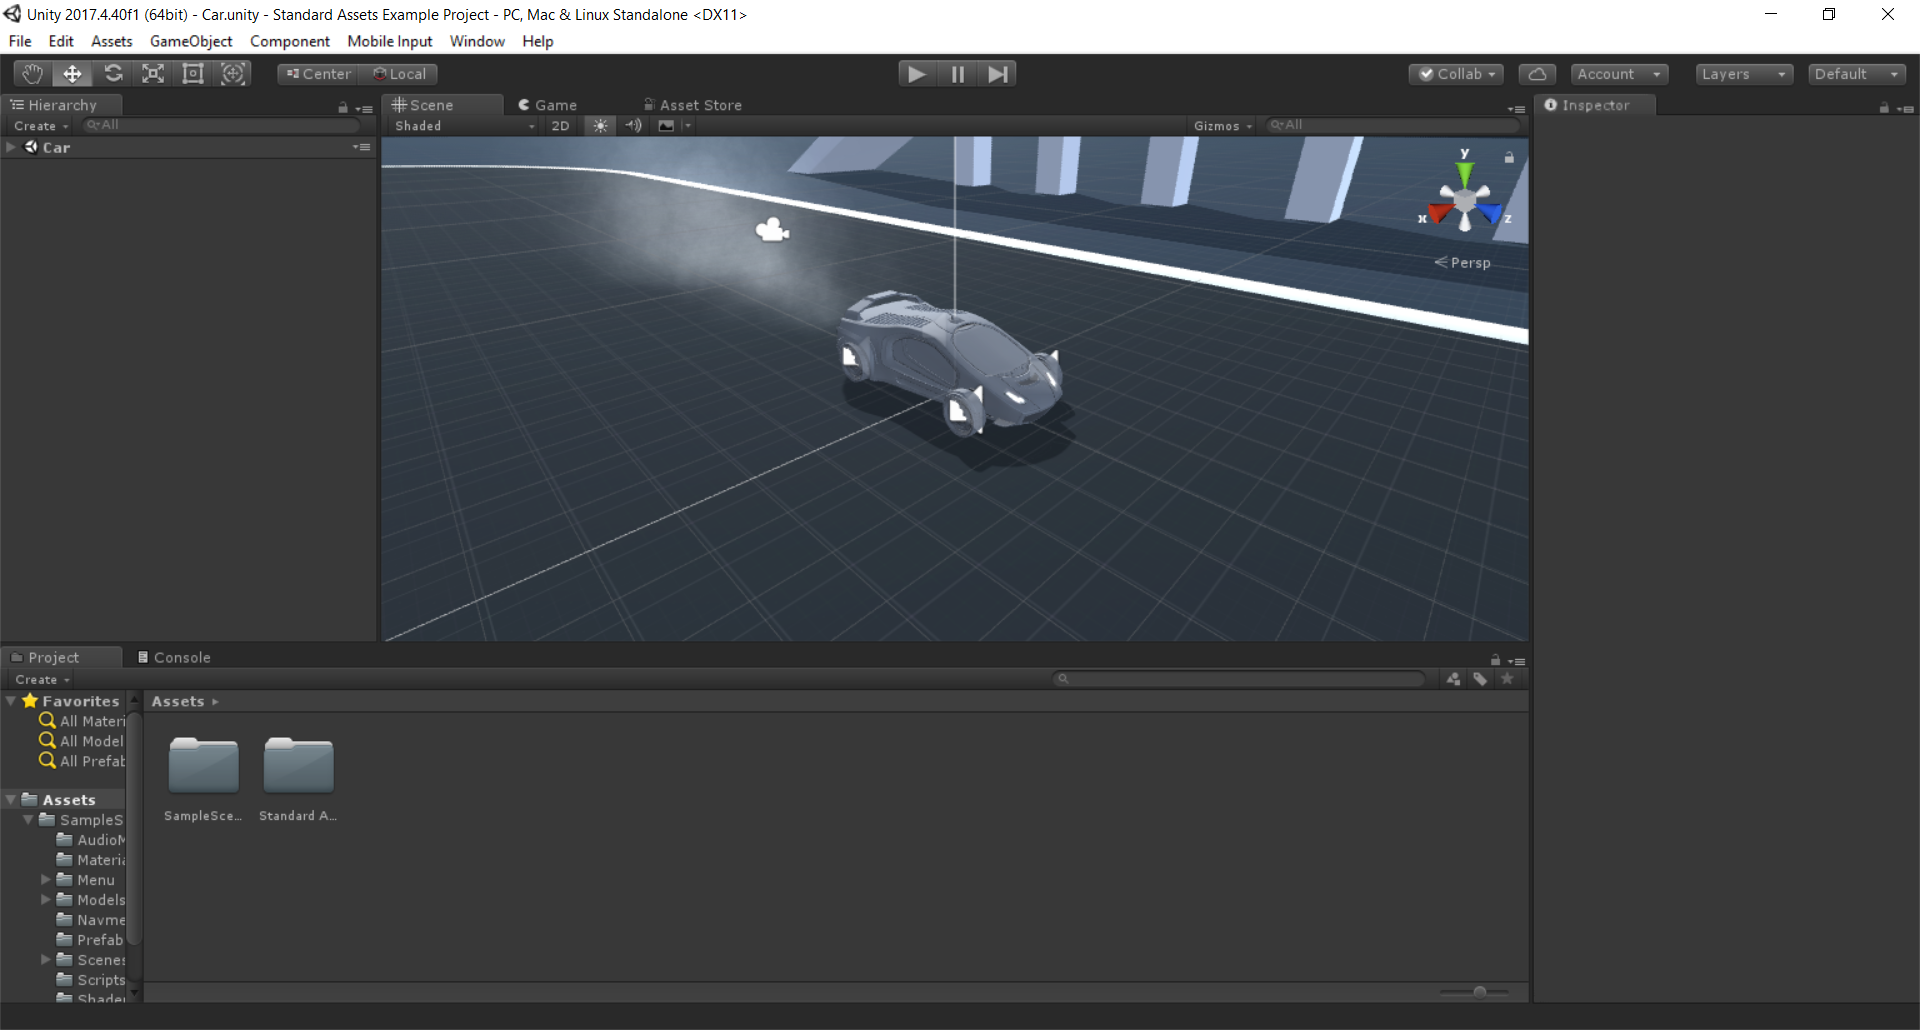
\includegraphics[width=\textwidth]{unity_default_layout.png}
\vspace{1pt}

I personally hate this layout (for the main reason that you can only see 4 panels at any given time which means you have to keep on switching between tabs). You can play around with this layout by simply dragging various tabs around the window to get the window configuration you like. I personally prefer this editor configuration, since now you can see all tabs within a single window:

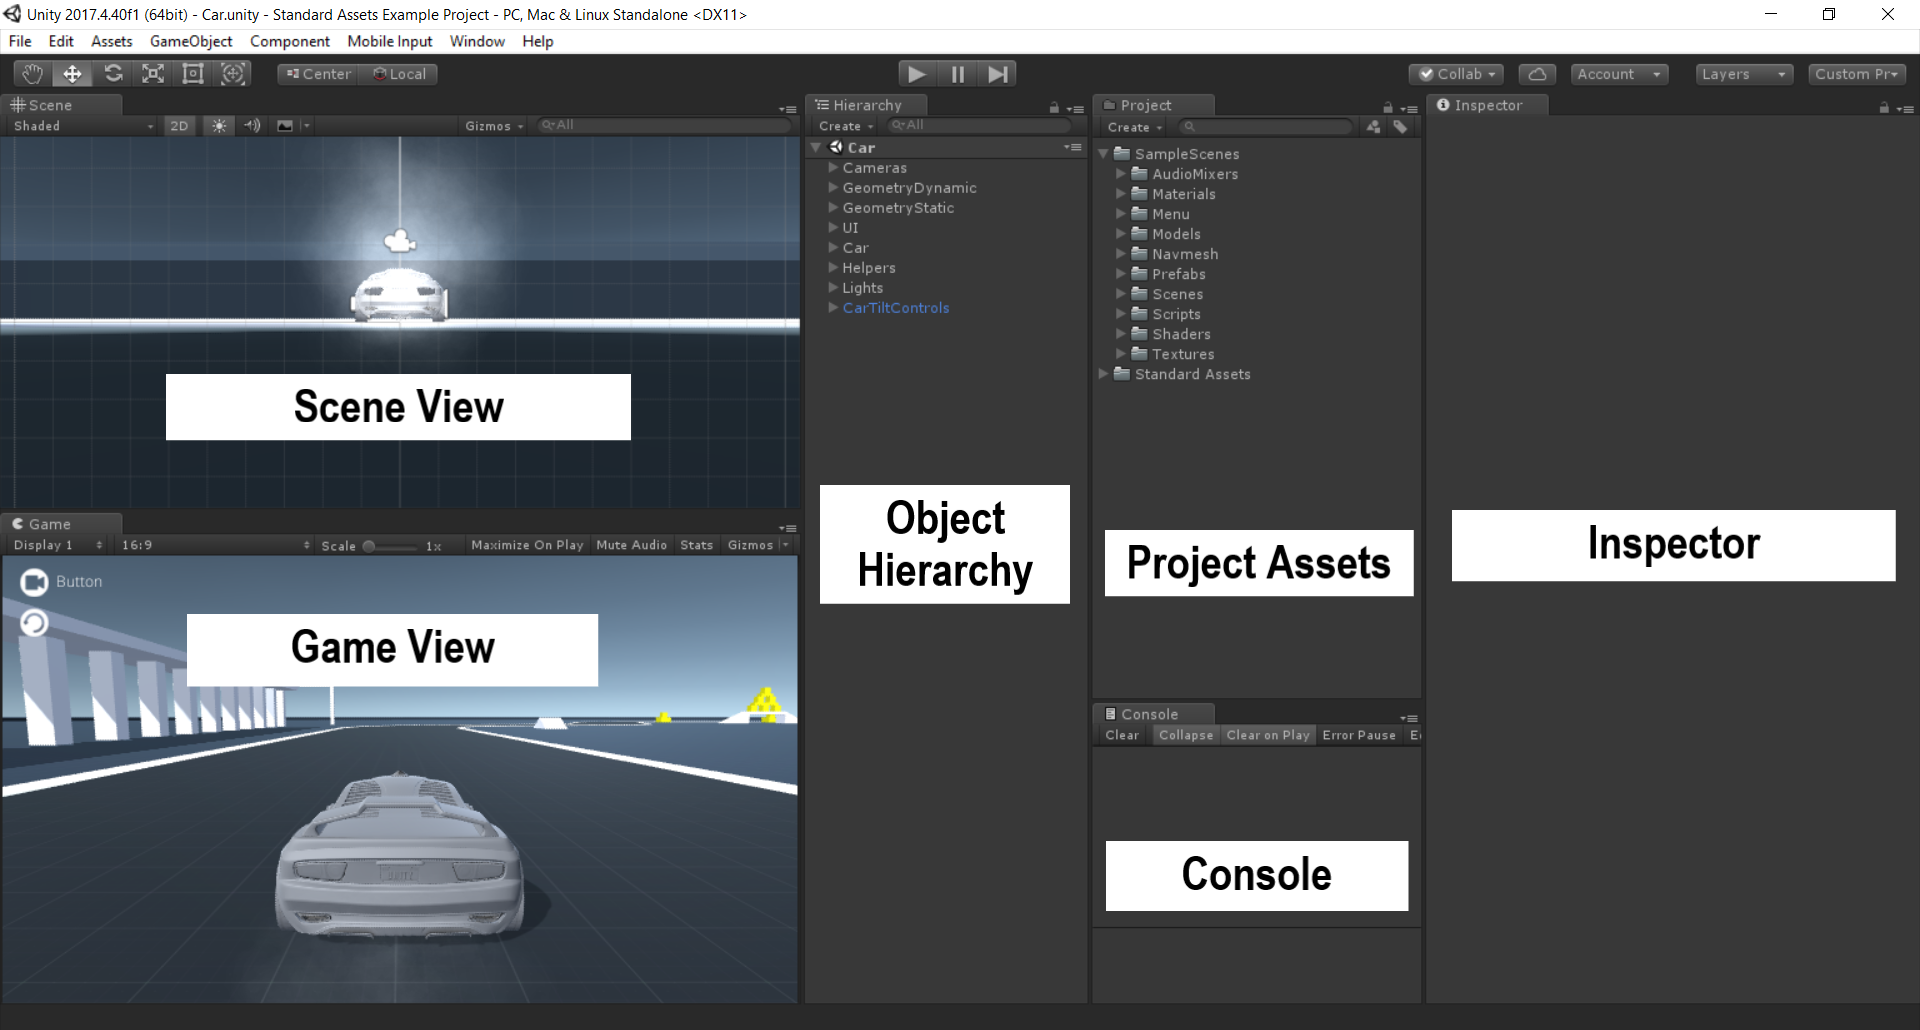
\includegraphics[width=\textwidth]{unity_custom_layout.png}
\vspace{1pt}

Let us now take a brief look at the various elements in the Unity3D interface:
\begin{itemize}
	\item Scene View: visual level editor for the currently open scene (edit mode)
	\item Game View: shows the view through the active camera object (the play button can be used to switch to play mode for playing and testing the game within the Unity editor)
	\item Object Hierarchy: hierarchical list of all game objects being used in the current scene along with parent-child relationships (is linked directly to the scene view)
	\item Project Assets: all the files and folders that make up the project (including the ones which are not being used in the current scene, but can be used later)
	\item Console: displays errors while building the scene (eg: lighting needs to be rebaked)
	\item Inspector: shows details of all game objects and components (like position, scale, scripts, materials, audio, etc) attached to them
\end{itemize}
You might now want to explore the Unity editor to look at various features. There are also many quick shortcuts in Unity that you can refer to here: \texttt{\href{https://docs.unity3d.com/Manual/UnityHotkeys.html}{https://docs.unity3d.com/Manual/UnityHotkeys.html}}.
\vspace{6pt}

\textbf{NOTE:} If you ever need to move/rename/delete asset files, do it in the Unity editor itself (in the Project Assets panel) and \textit{NOT} in the system file explorer - doing this may affect some connections between game objects and break your project.

\hrulefill
\pagebreak
\section{Basic Concepts}
\subsection{Game graphics concepts}
Before we start using Unity, let us briefly discuss the basics of computer graphics using the graphics display model:

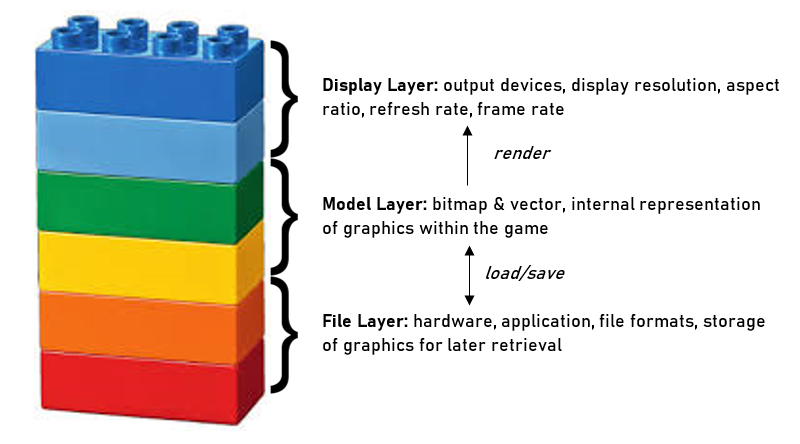
\includegraphics[width=\textwidth]{graphics_concepts.png}
\begin{enumerate}
	\item Display layer:
	\begin{itemize}
		\item display devices: laptop, smartphone, tablet, VR glasses
		\item display resolution: measure of how accurately a display approximates continuous images using finite pixels (pixel dimensions like 1920$\times$1080, dots/pixels per inch)
		\item aspect ratio: proportion of pixel map width vs height (eg: 1920$\times$1080 and 1280$\times$720 both have aspect ratio of 16:9)
		\item refresh rate: maximum rate at which the hardware can refresh the display image (expressed in hertz)
		\item frame rate: actual rate at which the hardware updates the display images (eg: a complex game might run at 60 FPS even though the display has a refresh rate of 240 Hz)
	\end{itemize}
	\item Model layer:
	\begin{itemize}
		\item bitmap image: stores color information about each individual pixel (zooming degrades image quality since we are not creating new pixels, but rather zooming in on the available pixels)
		\item vector image: stored internally as mathematical equations representing certain geometric aspects of the image (can be scaled up without loss of quality)
		\item vector images take longer to load (additional step of converting vector information to the corresponding pixel map before rendering it to the display), hence usually give lower frame rates
		\item 3D graphics: essentially vector graphics in 3 dimensions (i.e. 3D model defined by geometric polygons, usually triangles, to create a `mesh' of the model) - for realtime rendering at high FPS, we use low polygon modeling (i.e. limit number of polygons)
	\end{itemize}
	\item File layer:
	\begin{itemize}
		\item Unity supports nearly all file formats (support for 2D vector graphics also added recently)
		\item for 3D formats (eg: native Maya, 3ds Max, Blender files), Unity converts to FBX files while importing
	\end{itemize}
\end{enumerate}
\textbf{NOTE:} As a general rule of thumb, try to maintain highest achievable image quality for as long as possible - reduce it only if it is adversely affecting the gameplay.
\pagebreak
\subsection{Game audio concepts}
We can apply the analogy of the graphics display model here as well:
\begin{itemize}
	\item instead of the display we have a device which converts digital data signals back into analogue waves (7.1 surround system, headphones, etc)
	\item instead of image storage algorithms we have a process called sampling (approximation of continuous analogue input to discrete digital pulses)
	\item sample rate: number of times per second the sound wave is `sampled' (typically 44.1 kHz)
	\item sample size: amount of data stored per sample (typically 8, 16 or 32 bits)
	\item typical file formats include WAV, AIFF, OGG, MP3, etc (software like Adobe Audition or Audacity have their native file formats)
\end{itemize}
Audio is very important to games, and also one of the tougher things to actually make or synthesize digitally. There are 3 main types of game audio:
\begin{itemize}
	\item voice: easiest to come by - voice actors need not be professionals, they can be friends, family, etc (pro tip: keep background noise as low as possible, otherwise noise removal is a very difficult task in production)
	\item sound FX:
	\begin{itemize}
		\item[$-$] reactive FX: effects that occur as things happen in the game (royalty free, creative commons licensed effects can be easily found in places like the Unity Asset Store)
		\item[$-$] ambient FX: ambient noises that add a feeling of immersion (natural sounds often work better than digitized ambient effects)
	\end{itemize}
	\item music: adds emotional impact and complements the atmosphere (again free resources exist; commercially produced music will need you to buy a license in order that you do not violate copyright law)
\end{itemize}
\hrulefill
\begin{center}\textbf{END OF WEEK 1}\end{center}
This is the end of the documentation from Week 1 of the course. Continue reading forward for further weeks, or head over into Unity and try out some stuff yourself.

\hrulefill
\pagebreak
\section{Solar System Simulation}
While a solar system model is not technically a game, it is useful to start small and understand the basic workflow that goes into making a game. Sadly due to copyright issues, I am not sure if I can directly provide you the link to the project assets. In case you wish to follow along as I discuss the concepts, you might need to dig a little bit into my website github repository: \texttt{\href{https://github.com/omprabhu31/omprabhu31.github.io}{https://github.com/omprabhu31/omprabhu31.github.io}}.
\subsection{Importing assets into Unity}
To get started, launch Unity and create a new project (set the template as 3D and any location you prefer; no need to import standard assets) and extract the assets to a suitable location. To import the assets there are 2 methods:
\begin{itemize}
	\item Drag and drop the asset folders from the file explorer into the `Project' panel
	\item Click on the `Assets' tab $>$ Import New Asset... $>$ Browse each asset and add it
\end{itemize}
The first method is easier, especially in a big project where we have hundreds of individual asset files. Note that changes to assets within Unity will not affect the assets in the location you extracted them to. By now, you should have a screen that looks like this: 
\begin{center}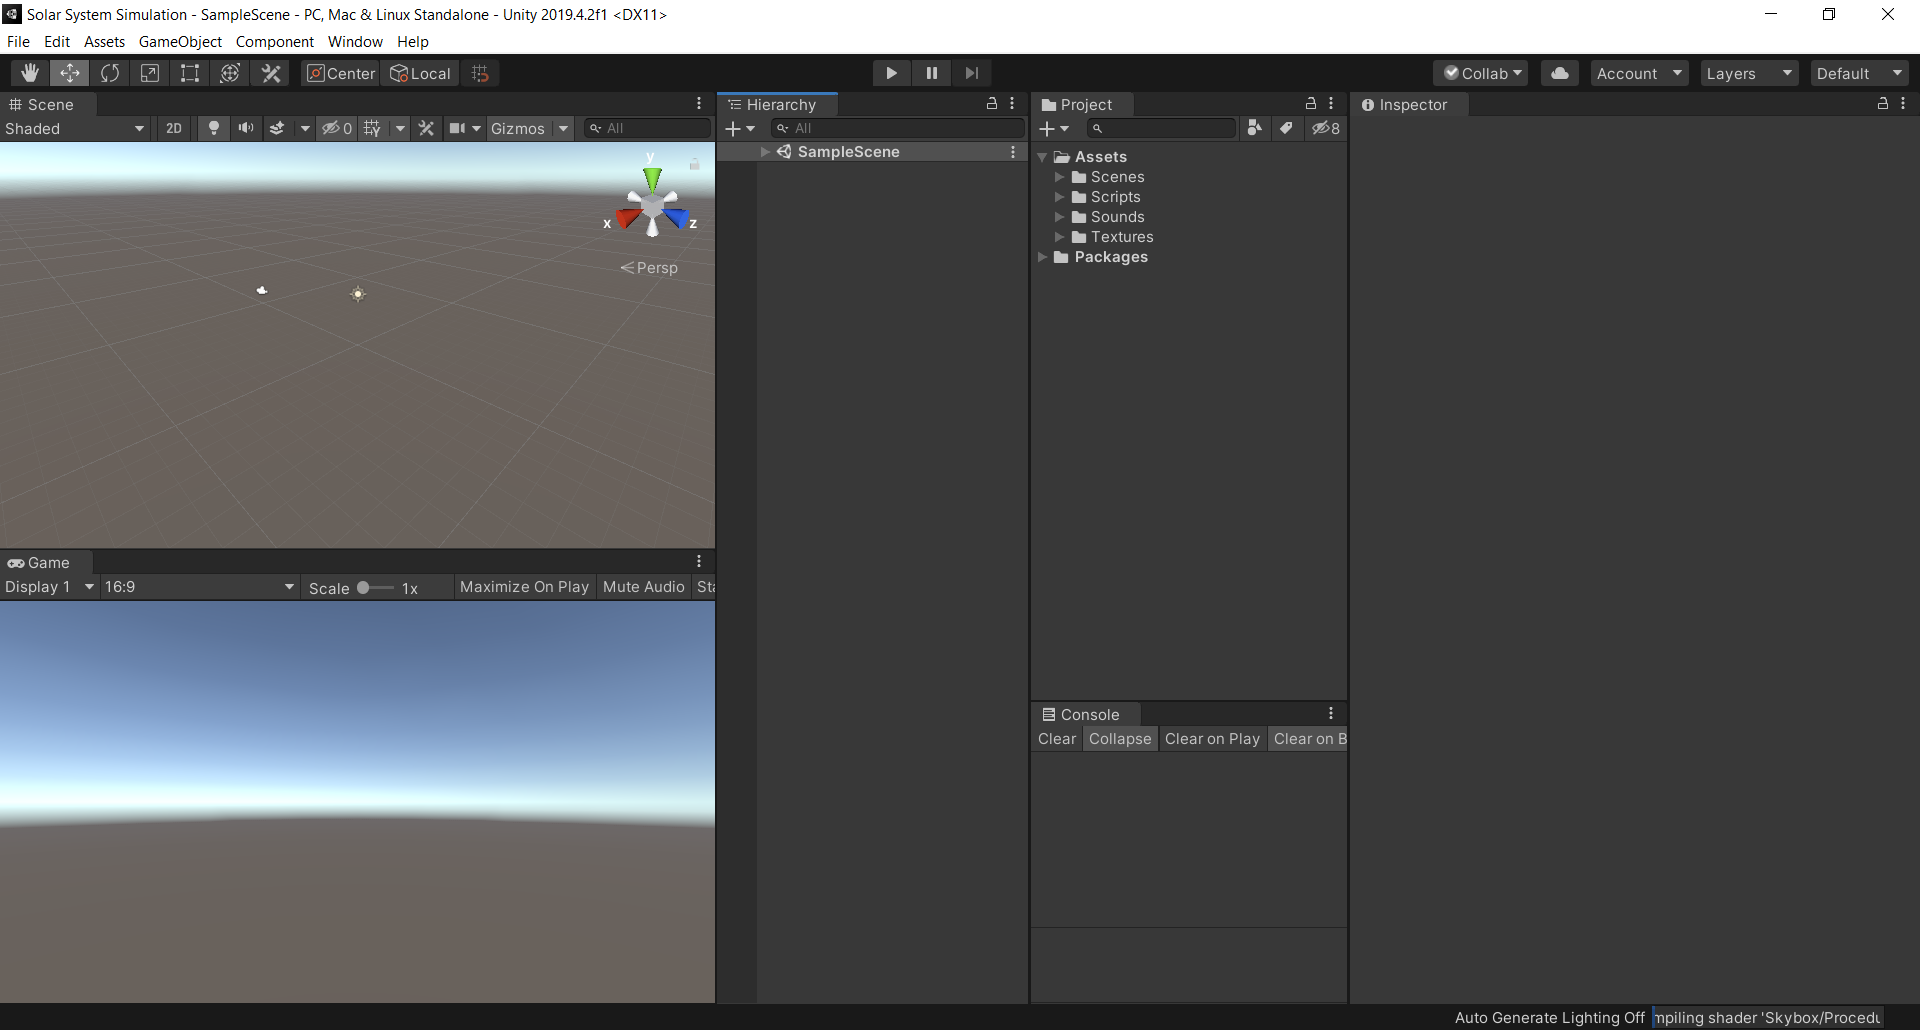
\includegraphics[width=\textwidth]{solarsystem_startscreen.png}\end{center}
We will be dealing with various game objects in a 3D cartesian system (pro-tip: to remember which axis is which colour, \textbf{RGB=XYZ}).
\subsection{Game objects and the transform component}

Now that we have a basic scene to work with, let's start out by adding the Sun, Earth and Moon as the first game objects. To do so, you might want to follow these steps (or maybe try to explore yourself how to do it):
\begin{enumerate}
	\item Click on the `GameObject' tab $>$ 3D Object $>$ Sphere
	\item In the `Inspector' panel, change the name of the object to `Sun'
	\item In the `Inspector' panel, adjust the position and scale parameters of the transform component
	\item Add the other 2 spheres, change their name, position and scale to suit them
\end{enumerate}
(If your game object initially appears in a weird position on your scene view, you can reset its transform by going to the `Inspector' panel $>$ right-click `Transform' $>$ Reset)
\vspace{6pt}

If you followed along these lines, you should have a screen that looks somewhat like this (could look slightly different based on the transform values you set):
\begin{center}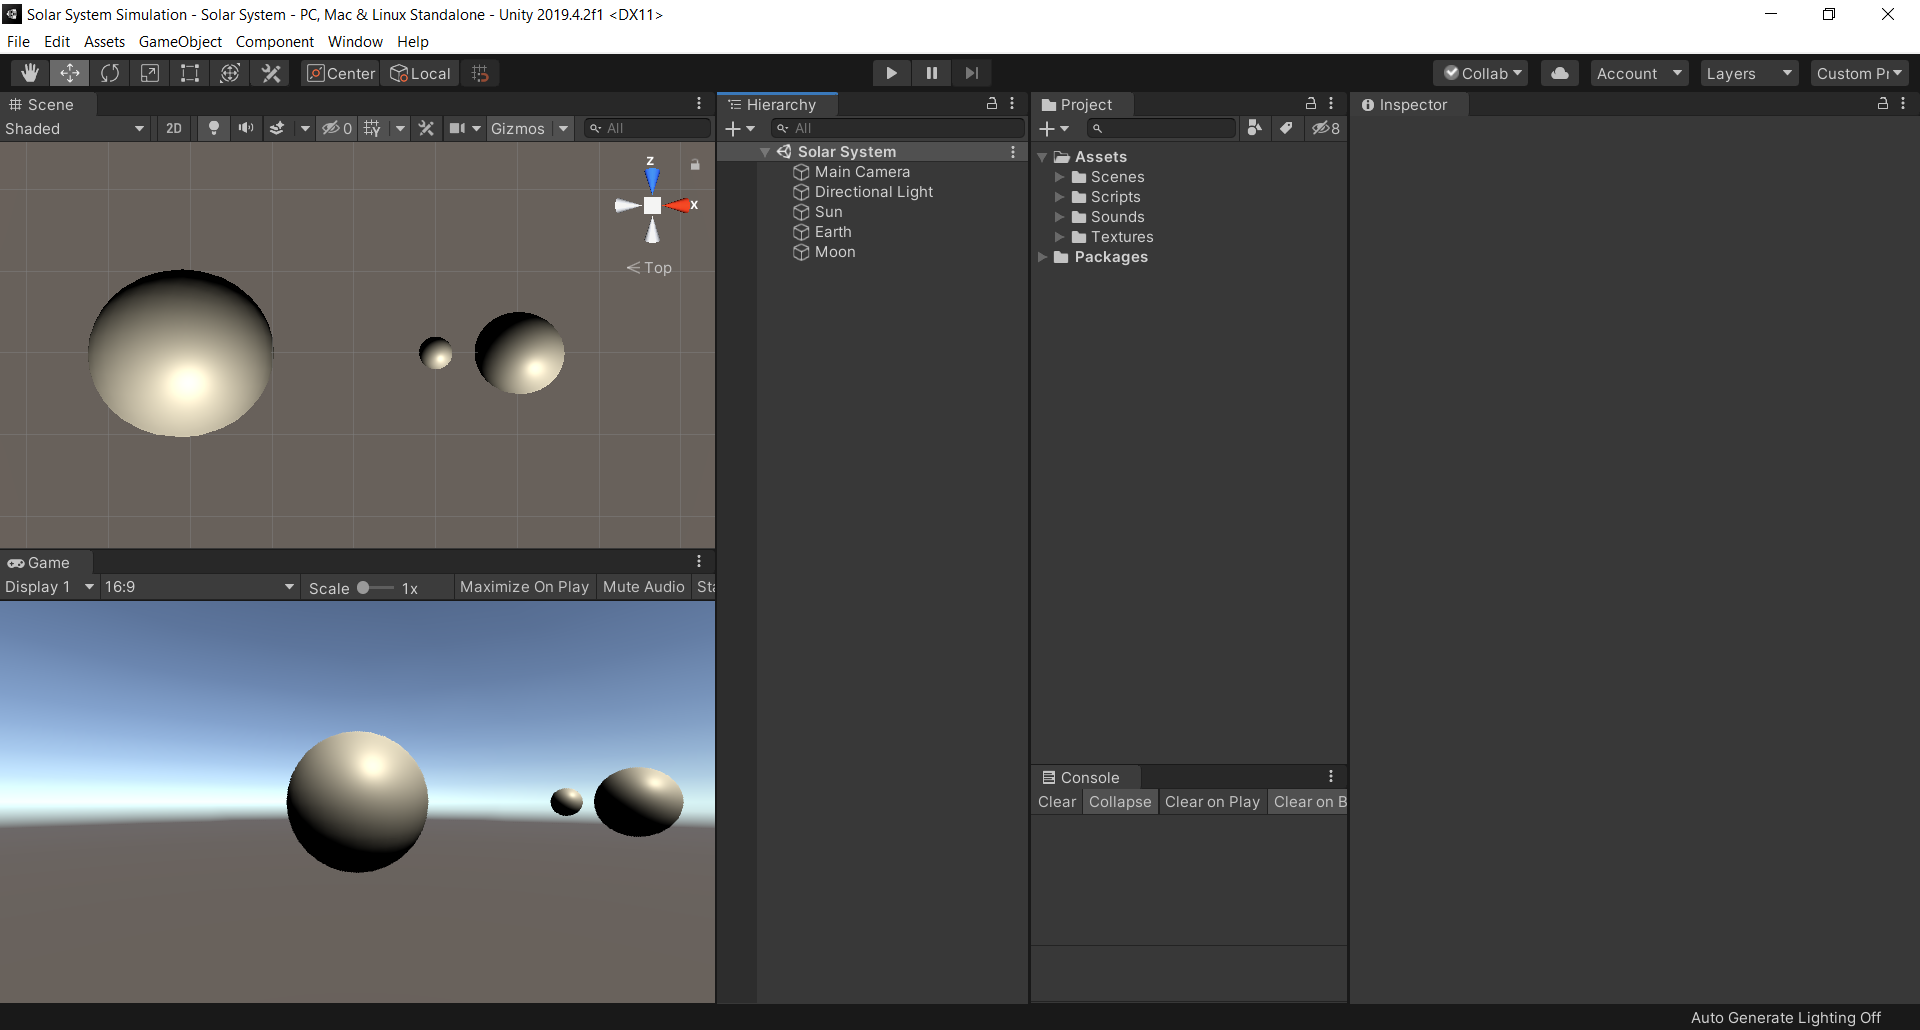
\includegraphics[width=\textwidth]{add_sun_earth_moon.png}\end{center}
As you can see, our objects have successfully been created in the `Hierarchy' panel and our scene and game views have been updated (Note: I have changed the position values in the transform component of the `Main Camera' object to focus the game view, however this is up to you).
\subsection{Adding behaviour to game objects}
Up till now, we have added the Sun, Earth and Moon as game objects. However, go into play mode and you will observe that they do not move. It is time to get them to rotate around each other appropriately. 
\vspace{6pt}

We do this by `adding behaviour' to our game objects. We do this through the use of scripts, which are nothing but files that contain code. This code tells Unity exactly how to get the game objects to behave with each other. Traditionally we would do this by writing the code ourselves, but as of now we have ready-made programs in the `Scripts' folder. From the names of the scripts, you might be able to (correctly) guess that we need to use the \texttt{RotateAround.cs} script here.
\subsubsection{Adding scripts}
Let us add the script to the Sun, Earth and Moon. Again there are multiple methods to add the script:
\begin{itemize}
	\item Click on the object in the hierarchy panel $>$ Click on `Add Component' in the inspector panel $>$ Click on `Scripts' $>$ \texttt{RotateAround.cs}
	\item Click \texttt{RotateAround.cs} in the projects panel $>$ drag and drop it on the desired game object
\end{itemize}
You will notice that a new `Rotate Around' component has been added into the inspector panel for the particular game object. It also contains two parameters - target (the object around which the selected game object will rotate) and speed (angular speed of rotation in degrees per second).
\vspace{6pt}

Note that the Earth rotates around itself as well as the Sun. This means we need to add the same script twice (similarly for the Moon as well).

\subsubsection{Adjusting script parameters}
Merely adding the script usually won't do anything. It is simply a component, and updating its parameter(s) is what will actually define the behaviour. I will elaborate the process for the `Earth' object, since there are 2 scripts we have to deal with:
\begin{enumerate}
	\item Target: drag and drop the `Sun' object onto target parameter of the first script in the inspector panel
	\item Speed: type in a suitable speed and test it in your game view and make further edits if any
	\item Similarly set up the second script by setting the target to the `Earth' object this time
\end{enumerate}
\begin{center}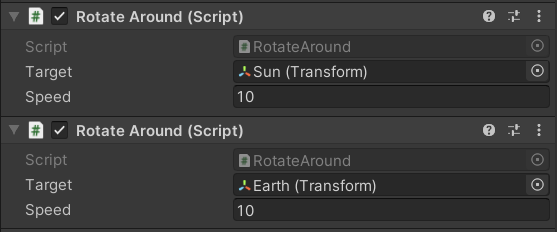
\includegraphics{rotatearound_earth.png}\end{center}
Complete these steps for the Sun and Moon as well (the Sun will need only one script, since it only rotates around itself), and please do not go into play mode yet. Note that there will not be any apparent effect of the objects rotating around themselves, but this is because we haven't added textures to them yet.
\subsubsection{Parent-child relationships}
Did you complete the above steps for the moon? Now go into play mode - I'm guessing you're having a pretty weird experience now. You're probably seeing the Moon chase the Earth and the distance between them increase. The reason for this delves a little bit into Mathematics and Physics, but I will discuss it in brief:
\begin{itemize}
	\item the \texttt{RotateAround.cs} script instructs the Moon to rotate around the `instantaneous center' of the Earth at any given point in time
	\item since the Earth is itself rotating around the Sun, the `instantaneous center' of the Earth is changing with time in the frame of reference of the scene view and so is the distance between the centers of the Earth and the Moon
	\item however, if we look from the frame of reference of the Earth (i.e. try to imagine that you're inside the Earth and at its center), what do you see? You will see apparently the Sun rotate around you, and the center of the Earth will appear stationary for you
\end{itemize}
If you still feel lost or get it partially, don't worry. You can look up the concept of `instantaneous center of rotation' on the internet and refer to some pretty good articles for more knowledge. 
\vspace{6pt}

Let's get back on track now. To fix this, we need to attach the Moon to the frame of reference to the Earth. In Unity language, we have to make the Moon a `child' of the Earth - this will make any motion of the Moon relative to the frame of the reference of the Earth. To do this, we simply click on the Moon in the hierarchy view and drag \& drop it onto the Earth.
\vspace{6pt}

Note that on setting the Moon as a child of the Earth, the transform components also change since the coordinates are now relative to the center of the Earth.
\subsection{Adding materials, lighting and audio}
\textit{(This sub-section is currently in the works. Expect it to be up in under a week's time.)}

\hrulefill
\pagebreak
\end{document}
